\subsection{Descripci\'on}

% Describir detalladamente el problema a resolver dando ejemplos del mismo y sus soluciones.

El sistema utilizado por Pascual consiste en cargar paquetes en camiones, de acuerdo al orden de llegada. Cada paquete se intenta cargar en el cami\'on con menor peso (con peso mayor que cero), si no es posible se guarda en un nuevo cami\'on.

El problema pide que se implemente el sistema utilizado por Pascual, con L (el peso m\'aximo soportado por todos los camiones), n (la cantidad de paquetes a cargar) y $p_1$, $p_2$, ..., $p_n$ (pesos de los paquetes) los par\'ametros de entrada.  Se supone que los paquetes no superan la capacidad m\'axima de los camiones.
Hagamos un ejemplo a modo de ilustraci\'on:

Sea L = 25, n = 7 y $p_1$ = 25, $p_2$ = 13, $p_3$ = 18, $p_4$ = 8, $p_5$ = 12, $p_6$ = 4 y $p_7$ = 1.
De acuerdo al m\'etodo del buen hombre, la soluci\'on es utilizar cuatro camiones con 25, 21, 18 y 17 sus pesos respectivos. El primer cami\'on contiene el primer paquete, el segundo cami\'on contiene al segundo y al cuarto paquete, el tercer cami\'on contiene el tercer paquete, el cuarto cami\'on contiene al quinto, sexto y s\'eptimo paquete.
Gráficamente:
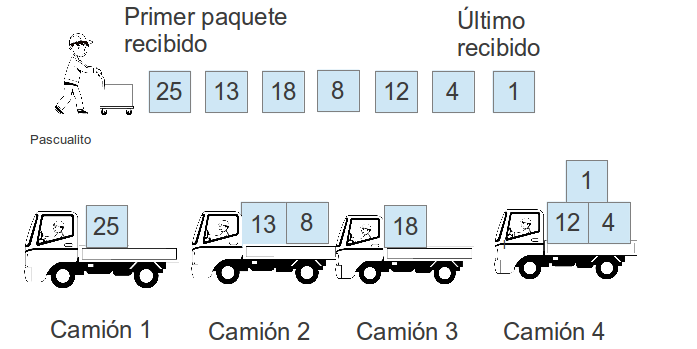
\includegraphics[scale=0.7]{ej1/Graficos/grafEj1.png} 

Para desarrollar un algoritmo que llegue a la misma soluci\'on que obtendr\'ia el sistema de Pascual, lo que hicimos fue seguir los mismos pasos que realiza dicho sistema. 
Para eso fue necesario reducir el enunciado a ciertos puntos b\'asicos, que nos llevar\'ian a la creaci\'on de nuestro modelo. 

Las caracter\'isticas del problema se reducen a lo siguiente:
\begin{itemize}
\item[1]- Los paquetes se encolan seg\'un el orden de llegada, por lo tanto el primer paquete que llega es el primero que se guarda en un cami\'on.
\item[2]- Siempre hay camiones disponibles, y todos ellos poseen el mismo l\'imite de carga.
\item[3]- Ning\'un paquete tiene un peso mayor al l\'imite de carga.
\item[4]- Se desea adem\'as conocer el n\'umero de camiones utilizados.
\item[5]- El m\'etodo de Pascual:
 Cada paquete intenta colocarse dentro de un cami\'on que ya est\'e con al menos una carga, Pascual intenta cargarlo en aquel que lleve menor peso, de no ser posible utiliza un nuevo cami\'on.
\end{itemize}